% !TeX spellcheck = en_US
\chapter{Business Plan}
	In this section we introduce our business idea and we describe our plan to introduce our product to the market. For this purpose, we analyze the current market situation by determining our clients and competitors, and describing the opportunities and threats that we see in the market. Also we describe the marketing strategy, that we will follow to reach our clients. Finally, we include a detailed overview of our capital costs calculation.

\section{Business Idea}
	uFixit is a platform for augmented reality user’s manuals. We will introduce our service to every company that has a hardware product with a user manual. Our goal is to equip each new hardware product with an augmented reality application, which represents a copy of the traditional owner manual. This application will help the user to install the product before the first use and to repair it in case of bugs. The augmented reality manual will be able to detect the problem in the product, search for a solution in the manual data base then guide the user through the repair steps. We will also offer the users the opportunity to make their own augmented reality repair tutorials. Then they will be able to share it with other users or include it in the original company’s manual, after it gets tested and approved by it. The company will be able to update the manual regularly with new fixes. 

\section{Clients}
	We can categorize our clients in 2 major groups: B2B and B2C. B2B clients are the companies producing the hardware, which we want to equip with the augmented reality user manual. These can be from different fields:  Automotive and mobility, smartphones and tablets, computers, domestic appliances, plant construction, industrial equipment… Each hardware producer can be a potential client. Our target clients are mostly the companies that thrive to optimize their after sales service. 
	\\
	\\
	B2C clients are the end users of the hardware products. A consumer in this case can be any individual that has access to an augmented reality capable device. This can be a smartphone, a tablet or augmented reality glasses. Our product is offered for both sexes and from the age of 12 years old. The Experts category can be an intersection of both clients’ categories. In fact, an expert can be an end user with advanced knowledge about the product, that allows him to create instruction sets for some bugs or a repair shop, which we consider as a B2B client.

\section{Competition}
	As competition we understand every augmented reality developer with a platform able to develop user manuals. Based on our market research, we defined two competitors, which already offered similar product:
	
\begin{itemize}
	\item The first is Vuforia, which is an augmented reality platform offering a powerful Software Development Kit. Its platform has more than 225000 registered developers and has more than 25000 apps \footnotemark. 
	\footnotetext{\url{http://www.hyundainews.com}}
It was a Hyundai partner by the development of its virtual owner’s manual, which was presented in Los Angeles Auto Show in January 2016. It is “the first mainstream automaker to launch an augmented reality owner’s manual app“ \footnotemark. 
\footnotetext{\url{http://www.vuforia.com}}
	\item The second competitor is RE’FLEKT which developed an augmented reality application for Bosch Flex-Inspect that was introduced in NADA ATD Convention and Expo 2014 in New Orleans. This product only shows a live diagnose of the examined car, which allows the user to detect the problems. 
\end{itemize}

	 Both introduced competitors have the advantage of the experience with the augmented reality applications. However, none of them have the same service that we plan to offer. In fact, our idea differs from Vuforia’s product in the sharing platform that we will build for the end users, where they can exchange their experiences with the different bugs and problems. Our platform will also offer standard tools for the development of the manuals. These can be used by any client regardless from the product that he wants to document. The difference to RE’FLEKT’s product is the added value that comes with the interactive repair steps, displayed after the diagnose is done and the problem has been defined. 
	 
\section{Market Situation: Opportunities and Threat}
The evaluation of the augmented reality market after defining our clients and competitors allows us to determine the points where we can see the opportunities to grow and predict the threats that we could face.
\\
	The augmented reality market is expected to have a big and fast expansion in the next few years thanks to several application fields of this technology. Its revenues are expected to exceed these of the virtual reality, as described in \autoref{fig:Augmented Reality Market Forecast}. In fact, Digi-Capital predicts it to reach $ \$120 $ billion by $2020$, $4$ times more than the virtual reality. Its fast growth rate is reflected by a forecasted $12.000\%$ increase of the revenues between $2016$ and $2020$. 
	
\begin{figure}[H]
		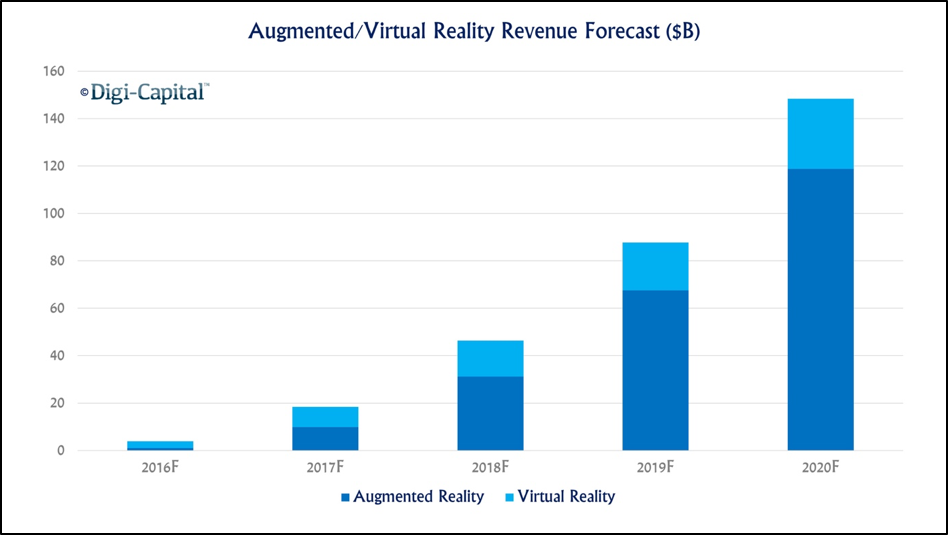
\includegraphics[width=\textwidth]{../images/ARrevenues.png}
		\centering
		\caption[Augmented Reality Market Forecast]{Augmented Reality Market Forecast\footnotemark}
		\label{fig:Augmented Reality Market Forecast}
\end{figure}
	\footnotetext{\url{http://www.digi-capital.com}}
	
	We see in this fast development rate good opportunity to start a new business, that we also expect to grow as fast as the augmented reality market. With our idea we intend to create a new market of virtual manuals. We will be able to draw the traits of this market and play a pioneer role in its expansion. The experience and client basis that we will acquire through this process is our biggest asset to face the emerging competition. \\
	\\
	However, we also identified some areas where we see important threats. We are aware about the volatility of the new market that we want to build. In fact, we cannot predict the reaction of the clients to the new idea. We intend to face this problem with a studied marketing strategy based on past experiences. With this strategy, which is described in the next section, we plan to reach a wide range of customers in an increment way. Experience sharing has been continuously increasing since the globalization brought by the internet and similar communication channels. Our vision is to be the green future of user manuals, as part of the digital transformation, which will be the trend of the next years, according to several studies. Another potential threat that we see is the slow development of the augmented reality technology, especially while dealing with complex problems such as the spatial and temporal registration issue. This can be resolved by increasing the research and innovation investment in this area. 
\begin{figure}[H]
		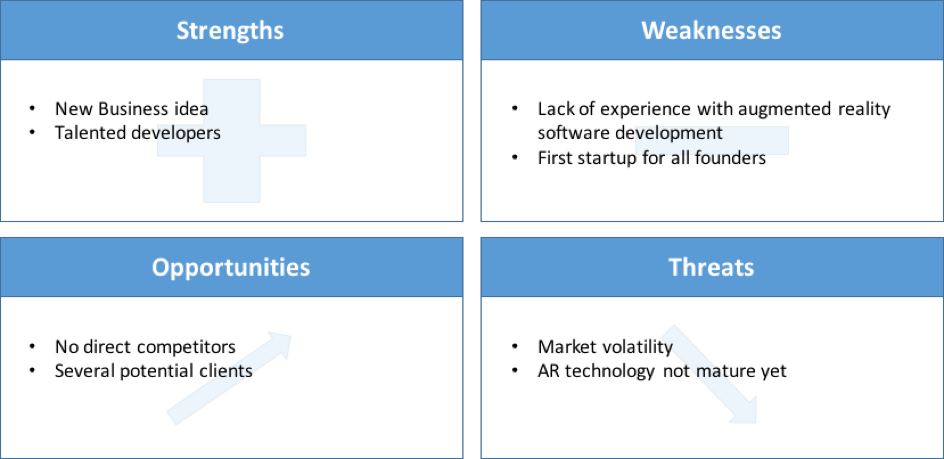
\includegraphics[width=\textwidth]{../images/SWOTanalysis.png}
		\centering
		\caption[Augmented Reality User Manual Market: SWOT Analysis]{Augmented Reality User Manual Market: SWOT Analysis}
		\label{fig:SWOT}
\end{figure}

\section{Road Map}
We plan to follow an incremented strategy while introducing our product to the market. In fact, we want to reach every client category in different steps. We have three main milestones in our plan, as described in \autoref{fig:Road Map}:

\begin{figure}[H]
		
\includegraphics[width=\textwidth]{../images/RoadMap.png}
		\centering
		\caption[uFixit Road Map]{uFixit Road Map}
		\label{fig:Road Map}
\end{figure}

\begin{itemize}
	\item First we will provide our service for end users and experts. They will use our app to create and follow simple augmented reality instruction sets. In this stage, our user manuals will be equipped with simple annotation elements, such as text or arrows.

	\item In a second step, we will provide a platform to integrate the 3D CAD models to our app. The manufacturers could use this service to create higher quality augmented reality user guides. This will enhance the quality of their after sales service for the existing or new products.
	
	\item Finally, our target is to build a fixer community where they can share not only their repairing experiences but also their feedback and opinion about the augmented reality user manuals. 
\end{itemize}

\section{Marketing Strategy}
We are aware that creating a new market and convincing our clients with the added value that our product offers, has to be addressed with a smart marketing strategy. 
	First, we intend to reach the end users, who are repairing their own hardware and who we like to call “Fixers”. We will offer an application where they can build their own augmented reality repair instruction manuals. The channels that we plan to use for this purpose are social media and internet forums. After building our Fixers basis, we intend to move to the next step in our road map. 
	We will reach the hardware producers to offer them a platform, where they can use their $3$D Models of their product to build augmented reality manuals. For this purpose, we will focus on exhibition and fairs events, together with the traditional advertising, such our website presence and the technical magazines.
	\begin{table}[H]
\caption[Marketing Expenses for the First 2 Years]{Marketing Expenses for the First 2 Years}
\label{tab:Marketing Costs}
\begin{center}
\begin{tabular}{|l|r|r|}
\hline 
Marketing channel & Costs & Costs for first $2$ years \\ 
\hline 
Branding & - & $3.500$ \euro \\ 
\hline 
Website & - & $4.500$ \euro \\ 
\hline 
Social media & $1.500$ \euro & $36.000$ \euro \\ 
\hline 
Content marketing & $1.500$ \euro & $36.000$ \euro \\ 
\hline 
Traditional advertising & $2.500$ \euro & $60.000$ \euro \\ 
\hline 
Events & $4.500$ \euro & $108.000$ \euro \\ 
\hline 
Total & $10.000$\euro & $248.000$ \euro \\ 
\hline 
\end{tabular} 
\end{center}
\end{table}
In \autoref{tab:Marketing Costs}, we calculate the marketing costs that we expect for the first two years. Our target is to reach a break-even-point in this period. We estimate the total marketing costs for this period by \euro $248.000$.
\begin{figure}[H]
		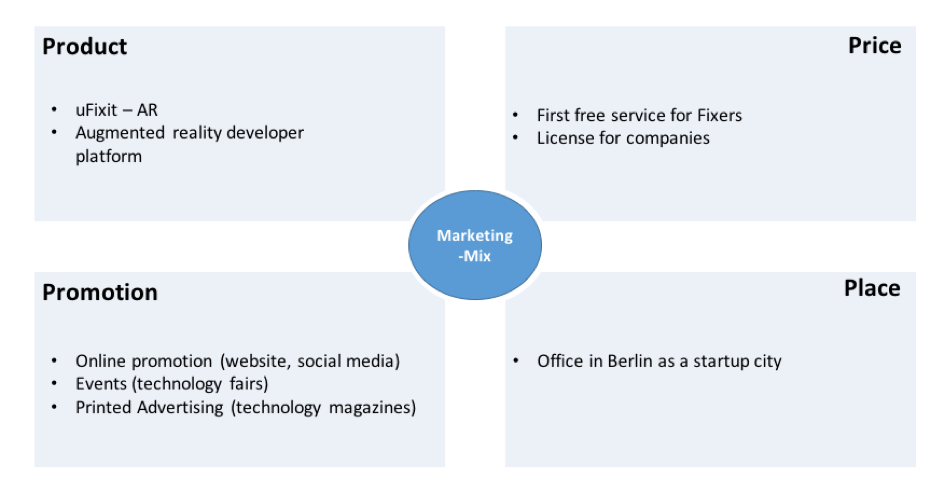
\includegraphics[width=\textwidth]{../images/MarketingStrategy.png}
		\centering
		\caption[uFixit Marketing Mix: $4$P's]{uFixit Marketing Mix: $4$P's}
		\label{fig:Marketing}
\end{figure}


\section{Capital Costs}
In this section we present our calculation for the capital costs, which we estimate based on present start-up founding costs and current market prices of promotion services, real estate, augmented reality hardware... This calculation, presented in the table TAB, also extends until the targeted break-even-point, and yields a total of \euro $422.510$, which we need to acquire in the first phase.

\begin{table}[H]
\caption[Capital Costs for the First 2 Years]{Capital Costs for the First 2 Years}
\label{tab:Capital Costs}
\begin{center}
\begin{tabular}{|l|r|}
\hline 
Capital costs & Costs for first 2 years \\ 
\hline 
Administrative founding costs & $100$ \euro \\ 
\hline 
Office & $56.000$ \euro \\ 
\hline 
Marketing & $248.000$ \euro \\ 
\hline 
AR Hardware & $40.000$ \euro \\ 
\hline 
Server \& other Hardware & $40.000$ \euro \\ 
\hline 
Total (incl.$10\%$ buffer) & $422.510$ \euro \\ 
\hline 
\end{tabular} 
\end{center}
\end{table}
